\documentclass[a4paper,12pt]{extarticle}
\usepackage[utf8x]{inputenc}
\usepackage[T1,T2A]{fontenc}
\usepackage[russian]{babel}
\usepackage[hidelinks]{hyperref}
\usepackage{indentfirst}
\usepackage{listings}
\usepackage{color}
\usepackage{here}
\usepackage{array}
\usepackage{multirow}
\usepackage{graphicx}
\usepackage{subcaption} 
\usepackage{mathtools}

\usepackage{caption}
\renewcommand{\lstlistingname}{Программа} % заголовок листингов кода

\bibliographystyle{ugost2008ls}

\usepackage{listings}
\lstset{ %
extendedchars=\true,
keepspaces=true,
language=C,						% choose the language of the code
basicstyle=\footnotesize,		% the size of the fonts that are used for the code
numbers=left,					% where to put the line-numbers
numberstyle=\footnotesize,		% the size of the fonts that are used for the line-numbers
stepnumber=1,					% the step between two line-numbers. If it is 1 each line will be numbered
numbersep=5pt,					% how far the line-numbers are from the code
backgroundcolor=\color{white},	% choose the background color. You must add \usepackage{color}
showspaces=false				% show spaces adding particular underscores
showstringspaces=false,			% underline spaces within strings
showtabs=false,					% show tabs within strings adding particular underscores
frame=single,           		% adds a frame around the code
tabsize=2,						% sets default tabsize to 2 spaces
captionpos=t,					% sets the caption-position to top
breaklines=true,				% sets automatic line breaking
breakatwhitespace=false,		% sets if automatic breaks should only happen at whitespace
escapeinside={\%*}{*)},			% if you want to add a comment within your code
postbreak=\raisebox{0ex}[0ex][0ex]{\ensuremath{\color{red}\hookrightarrow\space}},
texcl=true,
inputpath=listings,                     % директория с листингами
}

\usepackage[left=2cm,right=2cm,
top=2cm,bottom=2cm,bindingoffset=0cm]{geometry}

%% Нумерация картинок по секциям
\usepackage{chngcntr}
\counterwithin{figure}{section}
\counterwithin{table}{section}

%%Точки нумерации заголовков
\usepackage{titlesec}
\titlelabel{\thetitle.\quad}
\usepackage[dotinlabels]{titletoc}

%% Оформления подписи рисунка
\addto\captionsrussian{\renewcommand{\figurename}{Рисунок}}
\captionsetup[figure]{labelsep = period}

%% Подпись таблицы
%\DeclareCaptionFormat{hfillstart}{\hfill#1#2#3\par}
%\captionsetup[table]{format=hfillstart,labelsep=newline,justification=centering,skip=-10pt,textfont=bf}

%% Путь к каталогу с рисунками
\graphicspath{{fig/}}

%% Внесение titlepage в учёт счётчика страниц
\makeatletter
\renewenvironment{titlepage} {
 \thispagestyle{empty}
}
\makeatother

\DeclarePairedDelimiter\abs{\lvert}{\rvert}%
\DeclarePairedDelimiter\norm{\lVert}{\rVert}%

\usepackage{amsmath}

\begin{document}	% начало документа

% Титульная страница
\begin{titlepage}	% начало титульной страницы

	\begin{center}		% выравнивание по центру

		\large Санкт-Петербургский политехнический университет Петра Великого\\
		\large Институт прикладной математики и механики \\
		\large Кафедра <<Прикладная математика>>\\[6cm]
		% название института, затем отступ 6см
		
		\huge Математическая статистика\\[0.5cm] % название работы, затем отступ 0,5см
		%\huge Методы оптимизации\\[0.5cm] % название работы, затем отступ 0,5см
		\large \textbf{Отчет по лабораторной работе №4}\\[5.1cm]
		%\large \textbf{Отчет по лабораторной работе \\``Решение задач одномерной минимизации ``}\\[5.1cm]
		%\\[5cm]

	\end{center}


	\begin{flushright} % выравнивание по правому краю
		\begin{minipage}{0.25\textwidth} % врезка в половину ширины текста
			\begin{flushleft} % выровнять её содержимое по левому краю

				\large\textbf{Работу выполнил:}\\
				\large Колесник В.Н.\\
				\large {Группа:} 3630102/70201\\
				
				\large \textbf{Преподаватель:}\\
				\large к.ф.-м.н., доцент\\
				\large Баженов Александр Николаевич
				%\large Родионова Елена Александровна

			\end{flushleft}
		\end{minipage}
	\end{flushright}
	
	\vfill % заполнить всё доступное ниже пространство

	\begin{center}
	\large Санкт-Петербург\\
	\large \the\year % вывести дату
	\end{center} % закончить выравнивание по центру

\end{titlepage} % конец титульной страницы

\vfill % заполнить всё доступное ниже пространство


% Содержание
\renewcommand\contentsname{\centerline{Содержание}}
\tableofcontents
\newpage

\listoffigures
\newpage

\section{Постановка задачи}
Найти оценки коэффициентов линейной регрессии $y_i=a+bx_i+e_i$, используя 20 точек на отрезке [-1.8; 2] с равномерным шагом равным 0.2. Ошибку $e_i$ считать нормально распределённой с параметрами (0, 1). В качестве эталонной зависимости взять $y_i=2+2x_i+e_i$. При построении оценок коэффициентов использовать два критерия: критерий наименьших квадратов и критерий наименьших модулей. Проделать то же самое для выборки, у которой в значения $y_1$ и $y_{20}$ вносятся возмущения 10 и -10.

\section{Теория}
\subsection{Простая линейная регрессия}
\subsubsection{Модель простой линейной регрессии}
Регрессионную модель описания данных называют простой линейной регрессией, если
\begin{equation} \label{model}
y_i=\beta_0+\beta_1x_i+\varepsilon_i, i=1,...,n.
\end{equation}
где $x_1,...,x_n$ — заданные числа (значения фактора); $y_1,...,y_n$ — наблюдаемые значения отклика; $\varepsilon_1,...,\varepsilon_n$ — независимые, нормально распределённые $N(0,\sigma)$ с нулевым математическим ожиданием и одинаковой (неизвестной) дисперсией случайные величины (ненаблюдаемые); $\beta_0, \beta_1$ — неизвестные параметры, подлежащие оцениванию.\\
В модели (\ref{model}) отклик $y$ зависит зависит от одного фактора $x$, и весь разброс экспериментальных точек объясняется только погрешностями наблюдений (результатов измерений) отклика $y$. Погрешности результатов измерений $x$ в этой модели полагают существенно меньшими погрешностей результатов измерений $y$, так что ими можно пренебречь.

\subsubsection{Метод наименьших квадратов}
При оценивании параметров регрессионной модели используют различные методы. Один из наиболее распрстранённых подходов заключается в следующем: вводится мера (критерий) рассогласования отклика и регрессионной функции, и оценки параметров регрессии определяются так, чтобы сделать это рассогласование наименьшим. Достаточно простые расчётные формулы для оценок получают при выборе критерия в виде суммы квадратов отклонений значений отклика от значений регрессионной функции (сумма квадратов остатков):
\begin{equation} \label{ls}
Q(\beta_0, \beta_1)=\sum_{i=1}^{n}\varepsilon_i^2=\sum_{i=1}^{n}(y_i-\beta_0-\beta_1x_i)^2 \rightarrow \min_{\beta_0,\beta_1}.
\end{equation}
Задача минимизации квадратичного критерия (\ref{ls}) носит название задачи метода наименьших квадратов (МНК), а оценки $\widehat{\beta_0},\widehat{\beta_1}$ параметров $\beta_0, \beta_1$, реализующие минимум критерия (\ref{ls}), называют МНК-оценками.

\subsubsection{Расчётные формулы для МНК-оценок}
МНК-оценки параметров $\widehat{\beta_0}$ и $\widehat{\beta_1}$ находятся из условия обращения функции $Q(\beta_0, \beta_1)$ в минимум. Они равны:
\begin{equation} \label{beta1}
\widehat{\beta_1}=\frac{\overline{xy}-\overline{x}\cdot\overline{y}}{\overline{x^2}-(\overline{x})^2}
\end{equation}
\begin{equation} \label{beta0}
\widehat{\beta_0}=\overline{y}-\overline{x}\widehat{\beta_1}
\end{equation}

\subsection{Робастные оценки коэффициентов линейной регрессии}
Робастность оценок коэффициентов линейной регрессии (т.е. их устойчивость по отношению к наличию в данных редких, но больших по величине выбросов) может быть обеспечена различными способами. Одним из них является использование метода наименьших модулей вместо метода наименьших квадратов:
\begin{equation} \label{lad}
\sum_{i=1}^{n}|y_i-\beta_0-\beta_1x_i|\rightarrow\min_{\beta_0, \beta_1}
\end{equation}
Напомним, что использование метода наименьших модулей в задаче оценивания параметра сдвига распределений приводит к оценке в виде выборочной медианы, обладающей робастными свойствами. В отличие от этого случая и от задач метода наименьших квадратов, на практике задача (\ref{lad}) решается численно. Соответствующие процедуры представлены в некоторых современных пакетах программ по статистическому анализу.
Здесь мы рассмотрим простейшую в вычистлительном отношении робастную альтернативу оценкам коэффициентов линейной регрессии по МНК. Для этого сначала запишем выражения для оценок (\ref{beta1}) и (\ref{beta0}) в другом виде:
\begin{equation} \label{beta11}
\widehat{\beta_1}=\frac{\overline{xy}-\overline{x}\cdot\overline{y}}{\overline{x^2}-(\overline{x})^2}=\frac{k_{xy}}{s_x^2}=\frac{k_{xy}}{s_x s_y} \frac{s_y}{s_x}=r_{xy}\frac{s_y}{s_x},
\end{equation}
\begin{equation} \label{beta01}
\widehat{\beta_0}=\overline{y}-\overline{x}\widehat{\beta_1}
\end{equation}
В формулах (\ref{beta11}) и (\ref{beta01}) заменим выборочные средние $x$ и $y$ соответственно на робастные выборочные медианы med $x$ и med $y$, среднеквадратические отклонения $s_x$ и $s_y$ на робастные нормированные интерквартильные широты $q_x^\ast$ и $q_y^\ast$, выборочный коэффициент корреляции $r_{xy}$ — на знаковый коэффициент корреляции $r_Q$:
\begin{equation}
\widehat{\beta_{1R}}=r_Q \frac{q_y^\ast}{q_x^\ast},
\end{equation}
\begin{equation}
\widehat{\beta_{0R}}=med y -\widehat{\beta_{1R}} med x ,
\end{equation}
\begin{equation}
r_Q=\frac{1}{n}\sum_{i=1}^{n}sgn(x_i-med x)sgn(y_i -med y),
\end{equation}
\begin{equation}
q_y^\ast=\frac{y_{(j)}-y_{(l)}}{k_q(n)}, q_x^\ast=\frac{x_{(j)}-x_{(l)}}{k_q(n)}. 
\end{equation}
\begin{equation}
l=
\begin{cases}
[n/4]+1 \text{ при } n/4 \text{ дробном,}\\
n/4 \text{ при } n/4 \text{ целом}.\\
\end{cases}
\end{equation}
\begin{equation}
j=n-l+1
\end{equation}
\begin{equation}
sgn z =
\begin{cases}
1 \text{ при } z>0\\
0 \text{ при } z=0\\
-1 \text{ при } z<0\\
\end{cases}
\end{equation}
Уравнение регрессии здесь имеет вид
\begin{equation} \label{eq}
y=\widehat{\beta_{0R}}+\widehat{\beta_{1R}}x.
\end{equation}
Статистики выборочной медианы и интерквартильной широты обладают робастными свойствами в силу того, что основаны на центральных порядковых статистиках, малочувствительных к большим по величине выбросам в данных. Статистика выборочного знакового коэффициента корреляции робастна, так как знаковая функция sgn $z$ чувствительна не к величине аргумента, а только к его знаку. Отсюда оценка прямой регрессии (\ref{eq}) обладает очевидными робастными свойствами устойчивости к выбросам по координате $y$, но она довольно груба.


\section{Реализация}
Лабораторная работа выполнена с помощью встроенных средств языка программирования R в среде разработки RStudio. Исходный код лабораторной работы приведён в приложении.

\section{Результаты}
\subsection{Оценки коэффициентов линейной регрессии}
\subsubsection{Выборка без возмущений}
Критерий наименьших квадратов:
\begin{equation}
\widehat{a}\approx1.92
\end{equation}
\begin{equation}
\widehat{b}\approx1.89
\end{equation}
Критерий наименьших модулей:
\begin{equation}
\widehat{a}\approx1.71
\end{equation}
\begin{equation}
\widehat{b}\approx1.92
\end{equation}
\begin{figure}[!htb]
    \centering
    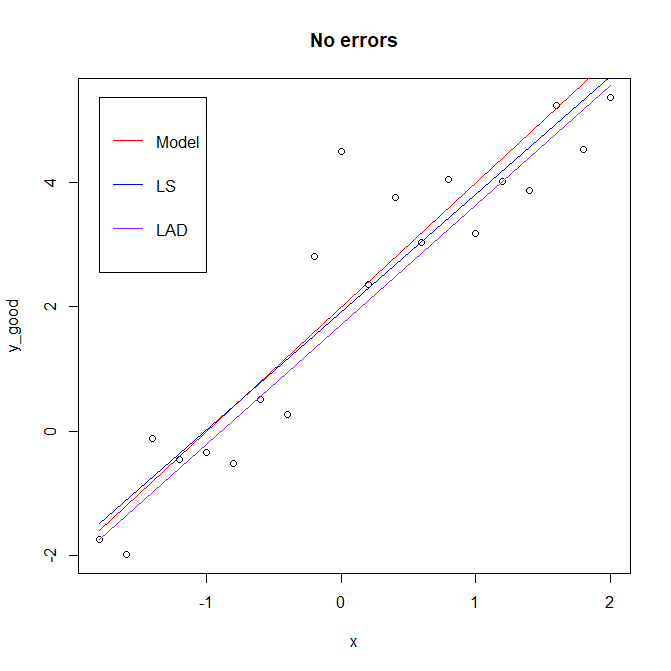
\includegraphics[width=0.5\textwidth]{no_errors}
    \caption{Без возмущений}
\end{figure}
\newpage
\subsubsection{Выборка с возмущением}
Критерий наименьших квадратов:
\begin{equation}
\widehat{a}\approx2.07
\end{equation}
\begin{equation}
\widehat{b}\approx0.46
\end{equation}
Критерий наименьших модулей:
\begin{equation}
\widehat{a}\approx1.78
\end{equation}
\begin{equation}
\widehat{b}\approx1.86
\end{equation}
\newpage
\begin{figure}[!htb]
    \centering
    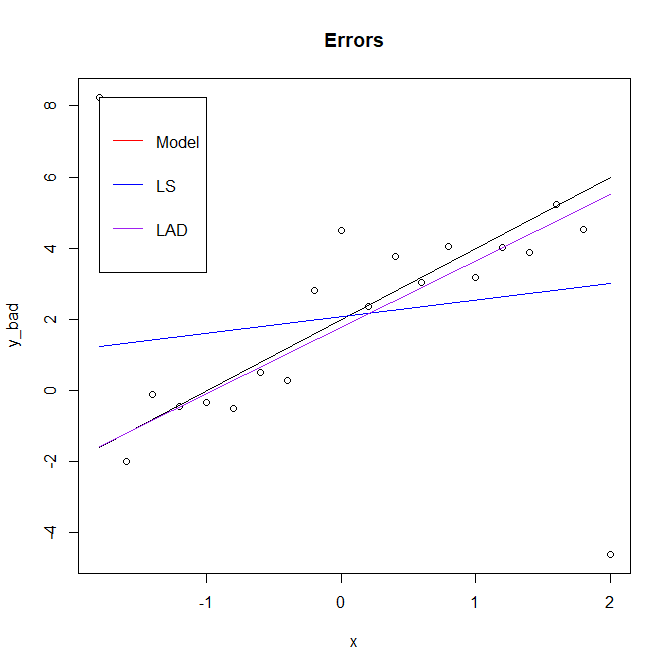
\includegraphics[width=0.5\textwidth]{errors}
    \caption{С возмущениями}
\end{figure}

\section{Обсуждение}
Рассмотрим пары чисел $(a,b)$ и $(\widehat{a},\widehat{b})$ как двумерные векторы. Оценим отклонение полученных результатов от эталонных по норме разности для выборки без возмущений. Для критерия наименьших квадратов по бесконечной норме получим 0.11, для критерия наименьших модулей - 0.29. Значит, критерий наименьших квадратов точнее оценивает коэффициенты линейной регрессии на выборке без возмущений.\\
Критерий наименьших модулей точнее оценивает коэффициенты линейной регрессии на выборке с возмущениями.\\
Критерий наименьших модулей устойчив к редким крупным выбросам.

\section{Приложения}
Репозиторий на Github с кодом лабораторной работы:\\
\url{https://github.com/VsevolodMelnikov/Math_Stat/tree/master/lab6}

\end{document}